\title{Eigenvalues and Eigenvectors}
\date{\today}

\documentclass[12pt]{article}
\usepackage{graphicx}
\usepackage{float}
\usepackage{hyperref}
\usepackage{cite}
\usepackage{subfig}
\usepackage{enumitem}
\usepackage{amsmath}
\usepackage{listings}
%\usepackage{fullpage}
%\bibliographystyle{science}
\bibliographystyle{plain}

\lstdefinelanguage{Maxima}{
  keywords={addrow,addcol,zeromatrix,ident,augcoefmatrix,ratsubst,diff,ev,tex,%
    with_stdout,nouns,express,depends,load,submatrix,div,grad,curl,%
    rootscontract,solve,part,assume,sqrt,integrate,abs,inf,exp},
  sensitive=true,
  comment=[n][\itshape]{/*}{*/}
}

\newif\ifanswers
%\answerstrue % comment out to hide answers

\begin{document}
\maketitle

\setcounter{equation}{0}
Ecologists often use ``Eigenvalues'' to determine the stability of multivariate dynamical systems. Eigenvalues are basically a simple summary of the long-term behavior of a system that is governed by a transition matrix. When they are negative around equilibria (or between -1 and 1 for discrete-time systems), this suggests that small perturbations away from the equilibrium will shrink back to the equilibrium as time goes on, and that the system is therefore locally stable.

\paragraph{} The more formal definition of Eigenvalues is often left somewhat mysterious. One of the useful formal explanations of what Eigenvalues actually do was given to my by Dr. Rehana Patel. Here, I will paraphrase her explanation, and in the process demonstrate the basic analytic methods for stability analysis.

At their simplest, matrices are simply a description of dynamics. Matrix multiplication can thus be used to apply transformations to a vector. As a simple example, consider a square in Cartesian space, with its corners at grid coordinates $\overrightarrow{v}_{1}=\{0,0\}$, $\overrightarrow{v}_{2}=\{0,1\}$, $\overrightarrow{v}_{3}=\{1,0\}$, and $\overrightarrow{v}_{4}=\{1,1\}$:

\begin{figure}[H]
  \centering
  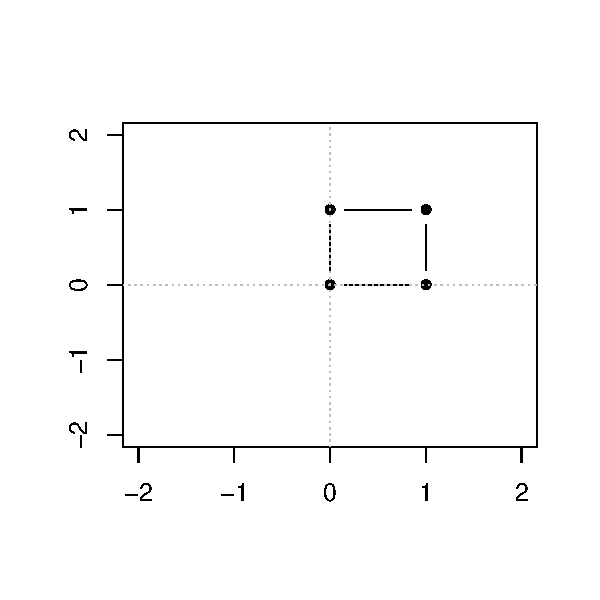
\includegraphics[width=0.5\textwidth, page=1]{figures/Eigen1}
\end{figure}

Now, try multiplying these grid coordinates by the following matrix:
\begin{equation}
\textbf{I}=
\begin{bmatrix}
1 & 0 \\
0 & 1
\end{bmatrix}
\end{equation}

You'll note that in all cases, $\textbf{I}\times\overrightarrow{v}_{i} = \overrightarrow{v}_{i}$. This is why we call \textbf{I} the ``Identity'' matrix -- just like multiplying a scalar by one returns the scalar, multiplying matrices by \textbf{I} returns the original matrix. Now, consider the reflection matrix:
\begin{equation}
\textbf{R}=
\begin{bmatrix}
0 & -1 \\
-1 & 0
\end{bmatrix}
\end{equation}

If we multiply the coordinates for the square by \textbf{R}, we now get $\textbf{R}\times\overrightarrow{v}_{1} = \{0,0\}$, $\textbf{R}\times\overrightarrow{v}_{2} = \{-1,0\}$, $\textbf{R}\times\overrightarrow{v}_{3} = \{0,-1\}$, and $\textbf{R}\times\overrightarrow{v}_{1} = \{-1,-1\}$. If we plot these new coordinates, we find that we have reflected the shape across the line $y=-x$:

\begin{figure}[H]
  \centering
  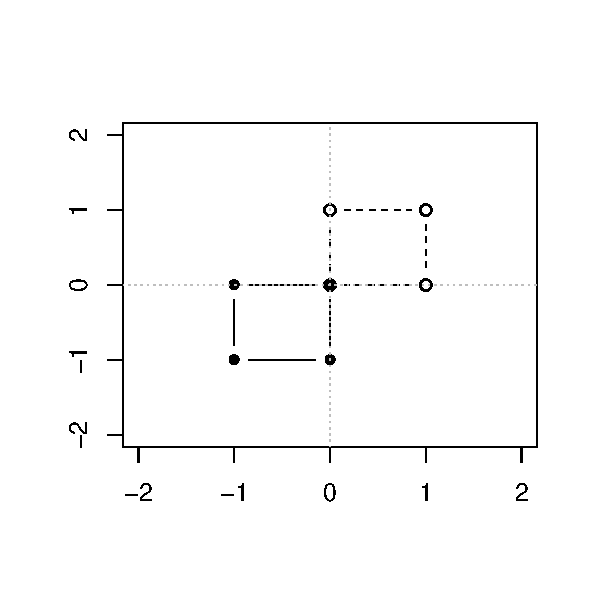
\includegraphics[width=0.5\textwidth, page=1]{figures/Eigen2}
\end{figure}

So, what do the Eigenvalues and Eigenvectors tell us in this case? Formally, Eigenvalues ($\lambda_{i}$) and Eigenvectors ($\overrightarrow{e_{i}}$) are defined for any matrix \textbf{M} such that $\textbf{M}\overrightarrow{e_{i}} = \lambda_{i}\overrightarrow{e_{i}}$ for all $i$. Here, $\lambda_{i}$ is a scalar. Thus, this formula states that we are looking for some vector that is not transformed when multiplied by matrix \textbf{M} -- rather, it should just change in magnitude by some fixed amount. For example, if $\overrightarrow{e_{i}} = \{2,1\}$, then we would expect that $\textbf{M}\times\overrightarrow{e_{i}} = \{2\lambda_{i},1\lambda_{i}\}$, rather than some other ratio, such as $\{1\lambda_{i},2\lambda_{i}\}$.

\paragraph{} To find Eigenvalues and Eigenvectors, we solve the system $det(\textbf{M}-\lambda\textbf{I})=0$, where \textbf{I} is the identity matrix, and $det$ signifies the determinant. For a 2-by-2 matrix (e.g. for \textbf{R}), the determinant is simply:
\begin{equation}
(\textbf{R}_{1,1} \textbf{R}_{2,2}) - (\textbf{R}_{2,1} \textbf{R}_{1,2})
\end{equation}

Thus, for \textbf{R}, we solve:
\begin{equation}
\begin{split}
det
\begin{bmatrix}
0-\lambda & -1 \\
-1 & 0-\lambda
\end{bmatrix}
= 0\\
(-\lambda)(-\lambda) - (-1)(-1) = 0\\
\lambda^{2} = 1\\
\lambda = \pm1\\
\end{split}
\end{equation}

To obtain the Eigenvectors, we substitute Eigenvalues back into the equation and solve for $(\textbf{M}-\lambda_{i}\textbf{I})\overrightarrow{e_{i}} = \overrightarrow{0}$, where $\overrightarrow{0}$ is a vector of zeros. Thus we solve:
\begin{equation}
\begin{split}
(\textbf{R}-(1)\textbf{I})\times\overrightarrow{e_{1}} = \overrightarrow{0}\\
\begin{bmatrix}
-1 & -1 \\
-1 & -1
\end{bmatrix}
\times\overrightarrow{e_{1}} = \overrightarrow{0}\\
\{-e_{1,1}-e_{1,2}, -e_{1,1}-e_{1,2}\} = \{0,0\}\\
e_{1,1}=e_{1,2}\\
(\textbf{R}-(-1)\textbf{I})\times\overrightarrow{e_{2}} = \overrightarrow{0}\\
\begin{bmatrix}
1 & -1 \\
-1 & 1
\end{bmatrix}
\times\overrightarrow{e_{2}} = \overrightarrow{0}\\
\{e_{2,1}-e_{2,2}, -e_{2,1}+e_{2,2}\} = \{0,0\}\\
e_{2,1}=-e_{2,2}\\
\end{split}
\end{equation}

Note that these vectors are described only in terms of relative magnitudes. By tradition, we scale these to sum to 1, such that $\overrightarrow{e_{1}}=\{1,1\}$ and $\overrightarrow{e_{1}}=\{1,-1\}$. Now, let's plot these vectors onto our Cartesian space:
\begin{figure}[H]
  \centering
  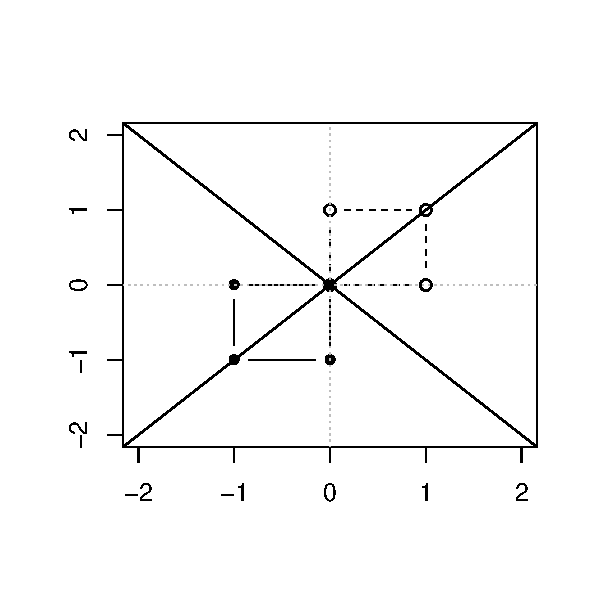
\includegraphics[width=0.5\textwidth, page=1]{figures/Eigen3}
\end{figure}

Note that, as expected, these vectors are not affected by the transformation imposed by matrix \textbf{R}. Consider the two points of the square that lie on the Eigenvectors ($\{0,0\}$ and $\{1,1\}$). Try flipping them over the line $y=-x$, and you will find that they remain on the vector before and after the transformation. Thus, the Eigenvectors show us directions of change which are not deformed by the transformation matrix.

So, what do the Eigenvalues show us? For this, let's imagine a transformation matrix described by $(2\textbf{R})$. This transformation still flips things over the line $y=-x$, but also doubles them in size:
\begin{figure}[H]
  \centering
  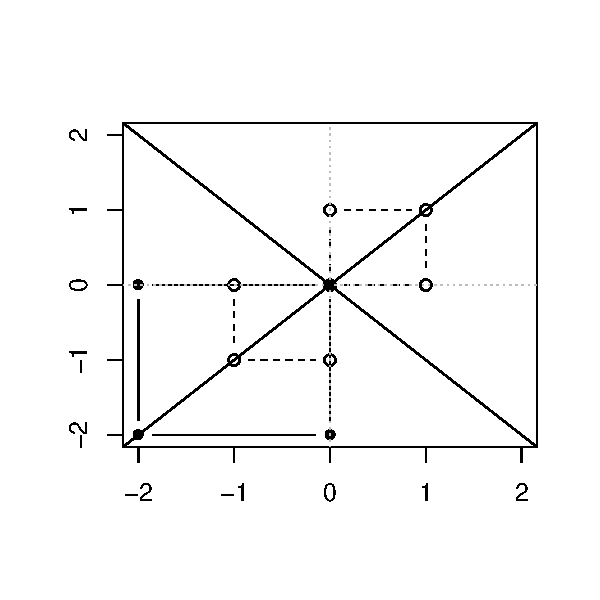
\includegraphics[width=0.5\textwidth, page=1]{figures/Eigen4}
\end{figure}

Note the points of the rectangle that fall along the Eigenvector $\{1,-1\}$ ($y=-x$). While the point $\{1,1\}$ does move as a result of the transformation to $\{-2,-2\}$, it doesn't change the relative magnitudes of its two components because it lies on an Eigenvector. However, it does change the total magnitude by a factor of two. If you try solving for the eigenvalues of $(2\textbf{R})$, you will find that $\lambda_{1}=2$ and $\lambda_{2}=-2$. Thus, the Eigenvalues show us the change in total magnitude caused by a matrix for points that fall along the Eigenvectors.

While this might seem somewhat abstract, it has a powerful implication for stability analysis. Consider a biological system that is influenced by a transformation matrix (e.g. a Leslie matrix, or a Jacobian matrix describing some continuous model near equilibrium). As we multiply the population vector by the same matrix many times, the matrix will cause transformations in all kinds of directions, that vary depending on the precise population values. However, any components of the transformation that fall along Eigenvectors will not be deformed by the matrix, and as the number of times you multiply the population vector by the matrix gets large, the influence of the Eigenvector will begin to swamp out other directions of change and come to dominate the overall population structure. Thus, the relative magnitude of items in the population vector (e.g. age classes in a Leslie matrix) will converge to the dominant Eigenvector (also known as the ``stable age distribution'').

Similarly, the Eigenvalues tells us whether changes get smaller or bigger through time. For continuous time systems, we consider a system at equilibrium to be locally stable if all Eigenvalues are less than $0$, as this tells us that changes in population size decrease as time goes on (thus, perturbations shrink to zero). For discrete time systems, Eigenvalues must be between $-1$ and $1$, because we track $N_{t+1}$, rather than $\frac{dN}{dt}$, as a function of $N_{t}$.

\end{document}